
\graphicspath{ {mainmatter/Bevilacqua_2007/} }
\title*{2007: Wireless Sensor Interface and Gesture-Follower for Music Pedagogy}
\titlerunning{Wireless Sensor Interface and Gesture-Follower} 
% if your contribution title if the original one is too long
\author{Frederic~Bevilacqua, Fabrice~Gu\'edy, Norbert~Schnell, Emmanuel~Fl\'ety, Nicolas Leroy}
\authorrunning{Bevilacqua et al.} %for an abbreviated version 
%%Norbert Schnell, Emmanuel Fl\'ety, Ircam-Centre Pompidou, STMS-Ircam-CNRS-UPMC \at STMS-Ircam-CNRS-UPMC, 1 place Igor Stravinsky 75004 Paris, France, \\ \email{\emph{firstname.lastname}@ircam.fr}
%\and Fabrice Gu\'edy \at current affiliation: Atelier des Feuillantines, Paris, France (was also with STMS-Ircam-CNRS at time of first publication), \email{Fabrice.Guedy@feuillantines.com}
%\and Nicolas Leroy \at  current affiliation: IPGP, Paris, France (was with Ircam-Centre Pompidou at time of first publication) \email{leroy@ipgp.fr}}
%
%
\maketitle

\abstract*{We present in this paper a complete gestural interface built to support music pedagogy. The development of this prototype concerned both hardware and software components: a small wireless sensor interface including accelerometers and gyroscopes, and an analysis system enabling gesture following and recognition. A first set of experiments was conducted with teenagers in a music theory class. The preliminary results were encouraging concerning the suitability of these developments in music education.}

\section{Introduction}

The recent developments in the fields of movement analysis and gesture capture technology create appealing opportunities for music pedagogy. For example, traditional instruments can be augmented to provide control over digital musical processes, altering standard instrument practice and offering potentially complementary pedagogical tools. Moreover, the development of novel electronic interfaces/instruments generates even more different paradigms of music performance, giving rise to potential novel approaches in music education. 

In this article we present a gestural interface that was integrated in a music education context. Both hardware and software components were developed and are described here. First, we report on the design of a relatively inexpensive miniature wireless sensor system that is used with accelerometers and gyroscopes. Second, we describe a gesture analysis system programmed in the Max/MSP environment to perform gesture recognition and following. The complete prototype enables us to experiment with various pedagogical scenarios. This research was conducted in the framework of the European I-MAESTRO project on technology enhanced learning, focusing on music education.\footnote{\url{http://www.i-maestro.org/}}

The motivation for this work is grounded in our pedagogical approach that considers physical gesture \cite{Iazzetta:2000} as a central element for performance but also for the embodiment of music concepts and theory. Our working hypothesis is that specific gestrual interactive systems can enhance this pedagogical approach. Even if similar or complementary tools have been already proposed and carried out \cite{Ferguson:2006,Guedy:2006,Lee:2006,Lee:2006a,Machover:2004,Puig:2005}, the use of digital technology and gestural interfaces in music pedagogy is at its very beginning.  Any use of new technology in music education represents difficult challenges, nevertheless we believe that such an approach offers great potential.

This paper is divided in three separate parts. The first two parts concern the technological developments, respectively the wireless sensor interface and the gesture follower/recognizer. In the third part, we present the pedagogical scenarios and the preliminary results we obtained after a first set of trials in music classes. 

\section{Wireless Interface and Sensors}

% Always give a unique label
% and use \ref{Bevilacqua:<label>} for cross-references
% and \cite{<label>} for bibliographic references
% use \sectionmark{}
% to alter or adjust the section heading in the running head
We developed and reported previously on several wireless interfaces, that were used in applications including the augmented violin project \cite{Bevilacqua:2006} and dance performances \cite{Flety:2005}. The experience we gained with these applications helped us to define requirements for the interface presented here.
\subsection{Requirements}
We developed in 2005 an 802.11b WiFi portable acquisition device called the WiSe Box \cite{Flety:2005}. An important advantage resides in the possibility of working simultaneously with multiple devices thanks to the different WiFi channels. The device offers 16 sensor channels, sampled on 16-bit resolution at 200 Hz sampling rate, for overall dimensions of $110\times65\times28$ mm. 
The aim of the development described here was to maintain most of the specifications of the WiSe Box while drastically reducing its size and power consumption. The following requirements were used as guidelines:

\begin{itemize}
\item compact size and weight enabling the sensors, wireless transmitter and battery to fit in a light handheld device
\item low power consumption, autonomy for standard rehearsal and performances
\item simultaneous use of multiple devices
\item low latency and sufficient accuracy  for music performance (typically sampled at 200 Hz on 10 bits).
\item cost effective
\item limited expertise and skills to operate the device. Robustness and reliability compatible within a pedagogical context.
 \end{itemize}

\subsection{Related works} 
Similar interfaces were reported recently. The company Infusion Systems proposes the Wi-microDig, a Bluetooth sensor interface.\footnote{\url{http://www.infusionsystems.com/}} The CrossBow company has a product line of MICA modules designed for sensor nodes to be spread in various distant locations in large space\footnote{Since the first publication in 2007, this company has significantly evolved, see \url{http://en.wikipedia.org/wiki/Crossbow\_Technology}.} Paradiso and coworkers at the MIT MediaLab developed a wireless and compact multi-user sensor system for dance performance featuring highly reduced size, high-end electronics and low-power supply solutions \cite{Aylward:2006}. Chou et al. developed at the University of California Irvine a thumb-sized sensor interface focused on node spreading.\footnote{\url{http://ecomote.net/}}

\subsection{Data acquisition and transmission}
We based our design on the XBee from MaxStream,\footnote{This model is not available anymore from this company, see the product evolution here \url{https://en.wikipedia.org/wiki/XBee}} which is a small form factor OEM module with simple communication means operating with the 802.15.4 IEEE standard (see Figure~\ref{Bevilacqua:fig1}). This standard, also known as Zigbee, is a variation of the 802.11 standard designed for embedded and low power wireless electronic devices. Most of the important features of a wireless network architecture are available: unique MAC address to identify each transceiver, beacon frames for node discovery and to wake up units in sleep mode, Carrier Sensing Multiple Access with Collision Avoidance (CSMA/CA) to share the bandwidth of a single frequency channel, and finally multiple channels over the ISM band.

\begin{figure}[t]
%\sidecaption
\center
% Use the relevant command for your figure-insertion program
% to insert the figure file.
% For example, with the graphicx style use
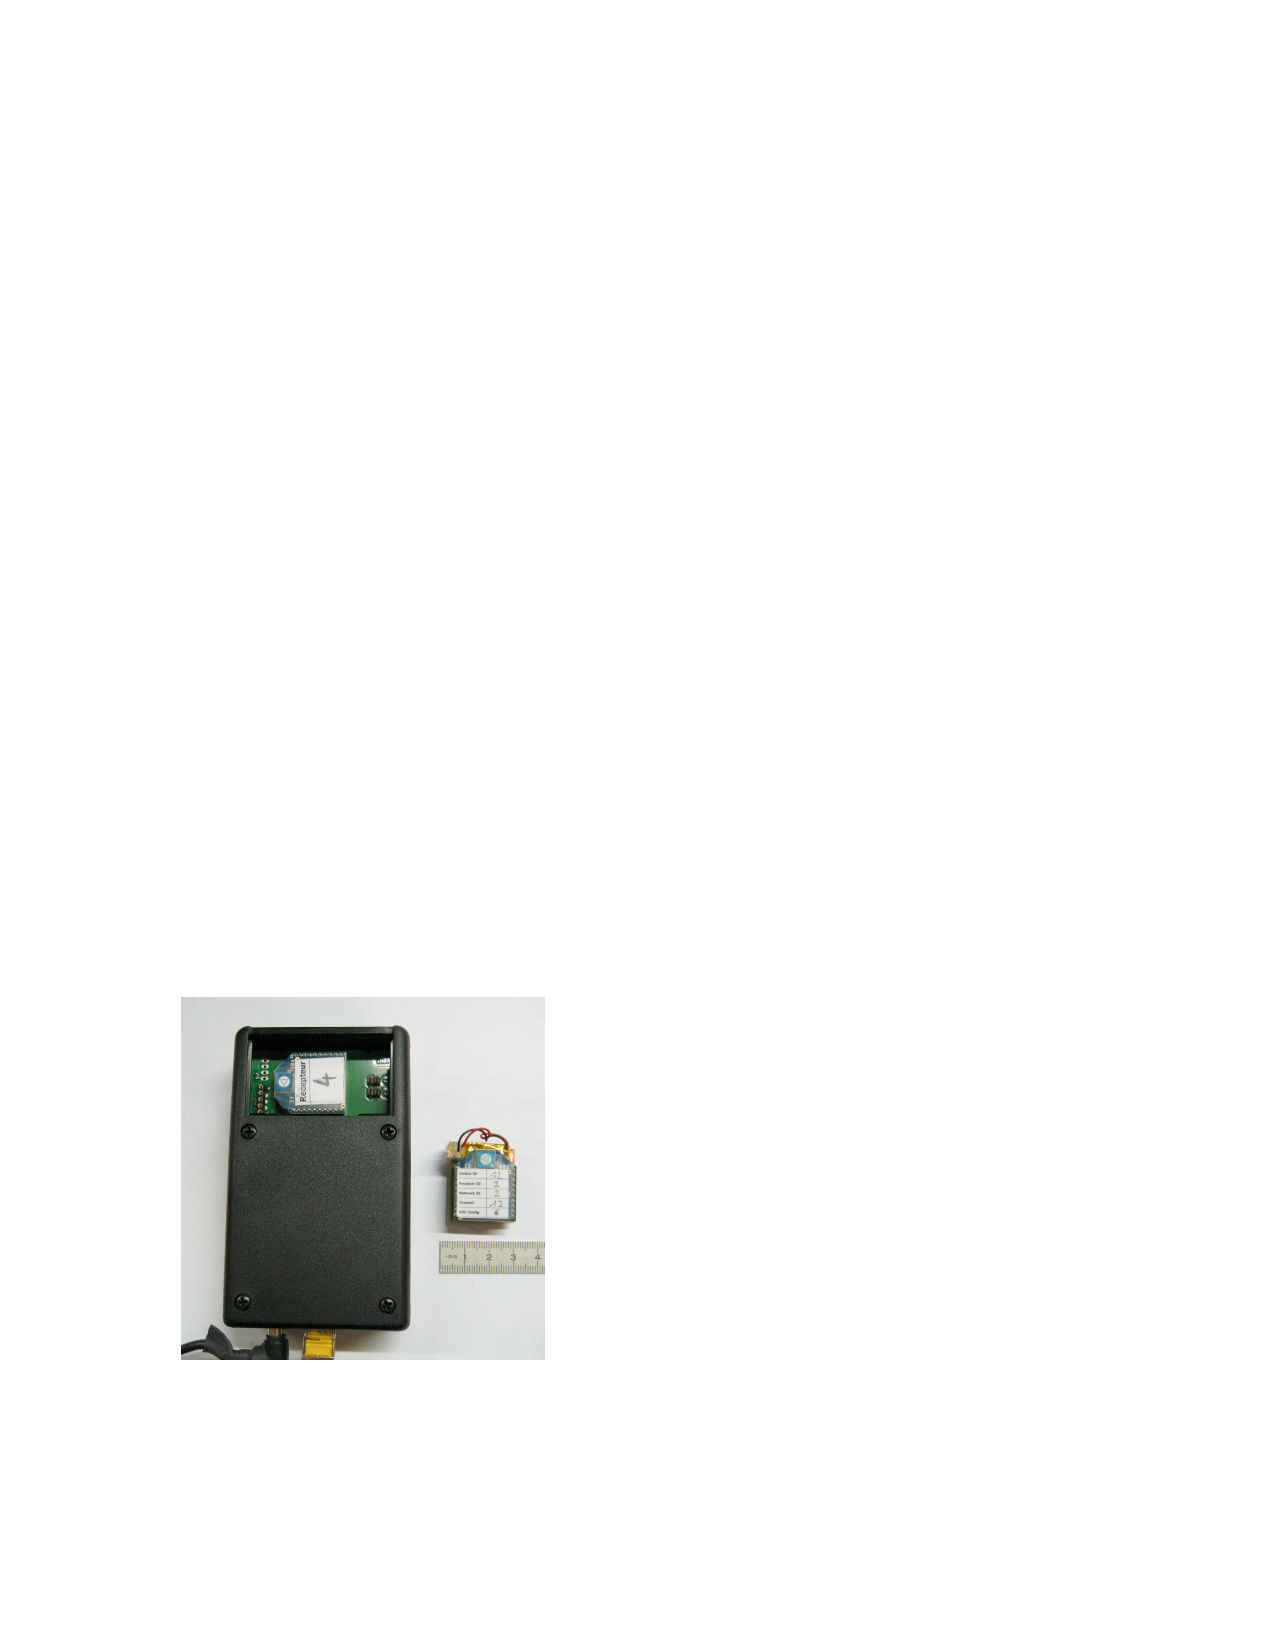
\includegraphics[scale=1.1]{fig1.pdf}
%
% If no graphics program available, insert a blank space i.e. use
%\picplace{5cm}{2cm} % Give the correct figure height and width in cm
%
\caption{Right: the module with Xbee, battery and sensors (on the back of the module). Left: receptor, showing the Ethernet and power supply connectors.}
\label{Bevilacqua:fig1}       % Give a unique label
\end{figure}

The XBee modules allow for the use of basic RS-232 wireless serial links to high-speed sensor networks. Each device can be considered as a serial modem (115200 bauds) and embeds a microcontroller that responds to AT commands for configuration and data transmission/reception. 
We used a specific version of the XBee module firmware that includes its own microcontroller operating the wireless section. The device features 6 analog inputs with a 10-bit AD converter. Thus, there is no need to use any additional microcontroller, and direct wiring of analog sensors to the XBee module is possible.

The CSMA/CA protocol allows for several transceivers to be merged into a single master but reducing the maximum data rate of each digitizer. To guarantee the highest data transmission performance, an individual receiver must be used for each emitter. 

\subsection{Data reception and computer communication}
The sensor data are sent as Open Sound Control messages over UDP, as often found in recent sensor digitizers such as the WiSe Box \cite{Flety:2005}, Toaster, the Kroonde \cite{Coduys:2004} or the Gluion.\footnote{\url{http://www.glui.de/}} The wireless receiver device uses a paired XBee module communicating with a PIC18F4520 Microchip microcontroller. The micro-controller communicates with the Microchip Ethernet controller ENC28J60 through a Serial Peripheral Interface (SPI) synchronous serial link. This enables the transmission of UDP packets with the OSC protocol. To reduce size and cost, we used a specific RJ-45 port containing both the link/data LEDs and the Ethernet isolation transformer. The data is received and processes by Max/MSP on the host computer connected to the receiver module.

\subsection{Sensors and power supply}
We choose a 5D Inertial Measuring Unit sensor including a ± 3g three-dimensional accelerometer from Analog Device (ADXL330) and an Invensense IDG-300 dual-axis gyroscope. Those two parts are available from Spark Fun Electronics\footnote{\url{https://www.sparkfun.com/}} assembled on a $22\times20$ mm Printed Circuit Board. 
For power supply, we chose a lithium-polymer flat battery of 3.6 volts / 140 mAh ($30\times20$ mm). This very small form factor allowed us to slide the battery between the main PCB and the XBee module, making the whole wireless module to fit a volume of $38\times27\times11$ mm. The overall device consumes 40 mA @ 2.8 volts and has an autonomy of 3 hours. If weight and size are not critical, a bigger battery might be used: we tested a 340 mAh model that last 7 hours. Note that one of the analog inputs can be used to monitor the battery voltage. 

\subsection{Performances and applications}
The sensor stream is digitized (10 bit) and transmitted at a framerate of 200 Hz for each emitter/receiver pair. Several modules can operate simultaneously. The range of the transmitter is 10 meters in an open area. This range may appear limited compared to usual OEM single RF frequency modules, but this does not represent a constraint for our applications where the receivers can be placed close enough to the emitter. If needed, larger range can be achieved by using the PRO version of the XBee modules, although autonomy might be reduced in such a case. 

The wireless sensor interface was fully tested and used in two applications: handheld devices for free gesture interaction and augmented string instruments (string quartet for example). This article concerns the first type of applications.

\section{Realtime Gesture Analysis}
%changed the order here of the begining (inversing frist two pargraphs)
In our context, a \emph{gesture} is defined by its numerical representation produced by the capture device. Technically, this corresponds to a multidimensional data stream, which can be stored in a matrix (e.g. row corresponding to time index, and column to sensor parameters). A multimodal ensemble of temporal curves can be directly accommodated within this framework, as long as all curves have identical sampling rate. 

\subsection{Gesture following/recognition}
The development of the \emph{gesture-follower} is pursued with the general goal to compare in real-time a performed gesture with a set of prerecorded examples, using machine learning techniques. Similar approaches have been reported \cite{Coduys:2004,Kolesnik:2004,Lee:2006,Lee:2006a,Merrill:2005,Pritchard:2006} and are often used in implicit mapping strategies.


\subsubsection{Following}
The \emph{gesture-follower} indicates, during the performance, the time location (or index) in relation to the recorded references. In other words, the \emph{gesture-follower} allows for the real-time alignment of a performed gesture with a prerecorded gesture. 

Figure~\ref{Bevilacqua:fig2} illustrates the computation, performed each time a new data is received, of the corresponding the time index of the reference. This operation can be seen as a real-time time warping of the performed gesture to the recorded reference. 

\begin{figure}[t]
%\sidecaption
\center
% Use the relevant command for your figure-insertion program
% to insert the figure file.
% For example, with the graphicx style use
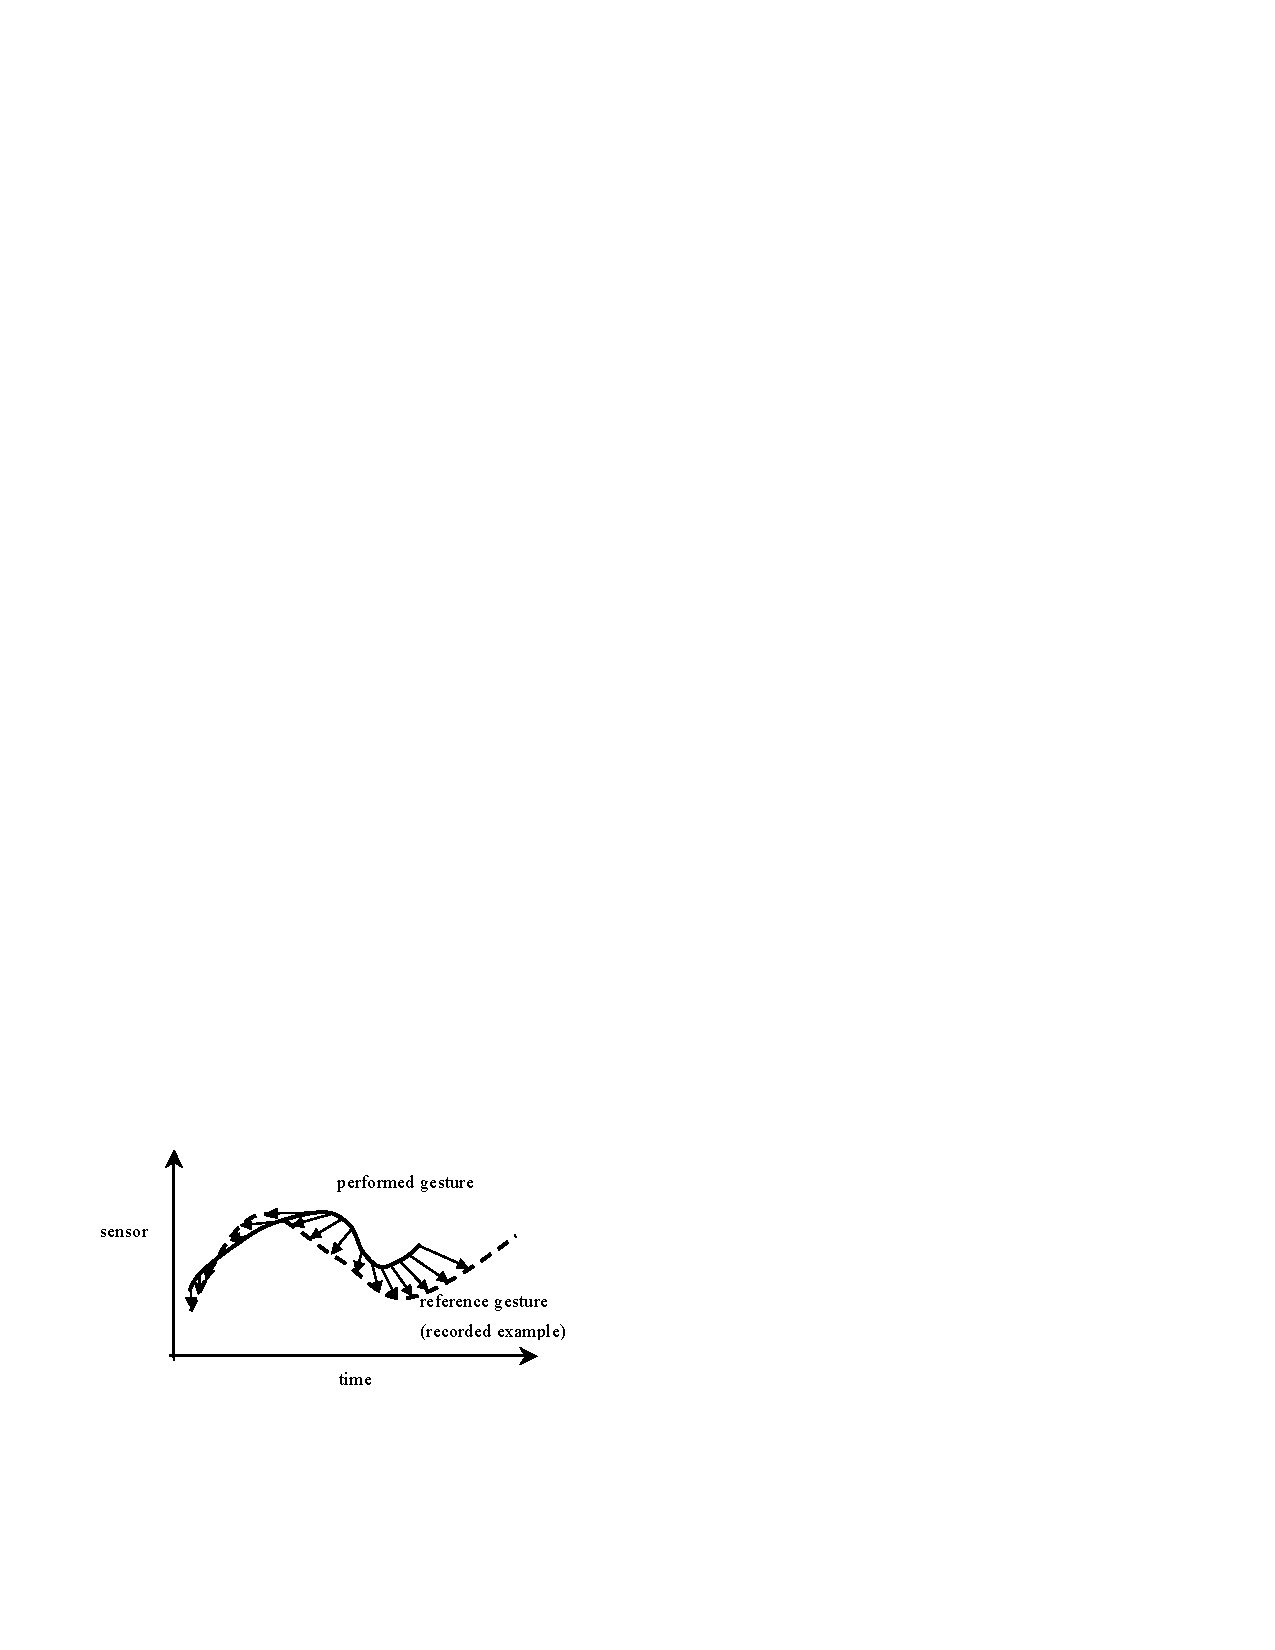
\includegraphics[scale=1.1]{fig2.pdf}
%
% If no graphics program available, insert a blank space i.e. use
%\picplace{5cm}{2cm} % Give the correct figure height and width in cm
%
\caption{The following paradigm: the performed gesture is time warped to a given reference.}
\label{Bevilacqua:fig2}       % Give a unique label
\end{figure}

\subsubsection{Comparing and recognising}
The process explained in the previous section can be performed with several references simultaneously. In this case, the system computes also the likelihood values for each reference to match the performed gesture. An example of this process is illustrated in Figure~\ref{Bevilacqua:fig3}  where the performed gesture is compared to two other examples. 

As shown in Figure~\ref{Bevilacqua:fig3} the likelihood values are updated continuously while the performed gesture is unfolding. The result of the recognition can therefore vary from the beginning, middle or the end of the performed gesture. Gesture recognition can be achieved by simply selecting the highest likelihood, at a chosen time.

\begin{figure}[t]
%\sidecaption
\center
% Use the relevant command for your figure-insertion program
% to insert the figure file.
% For example, with the graphicx style use
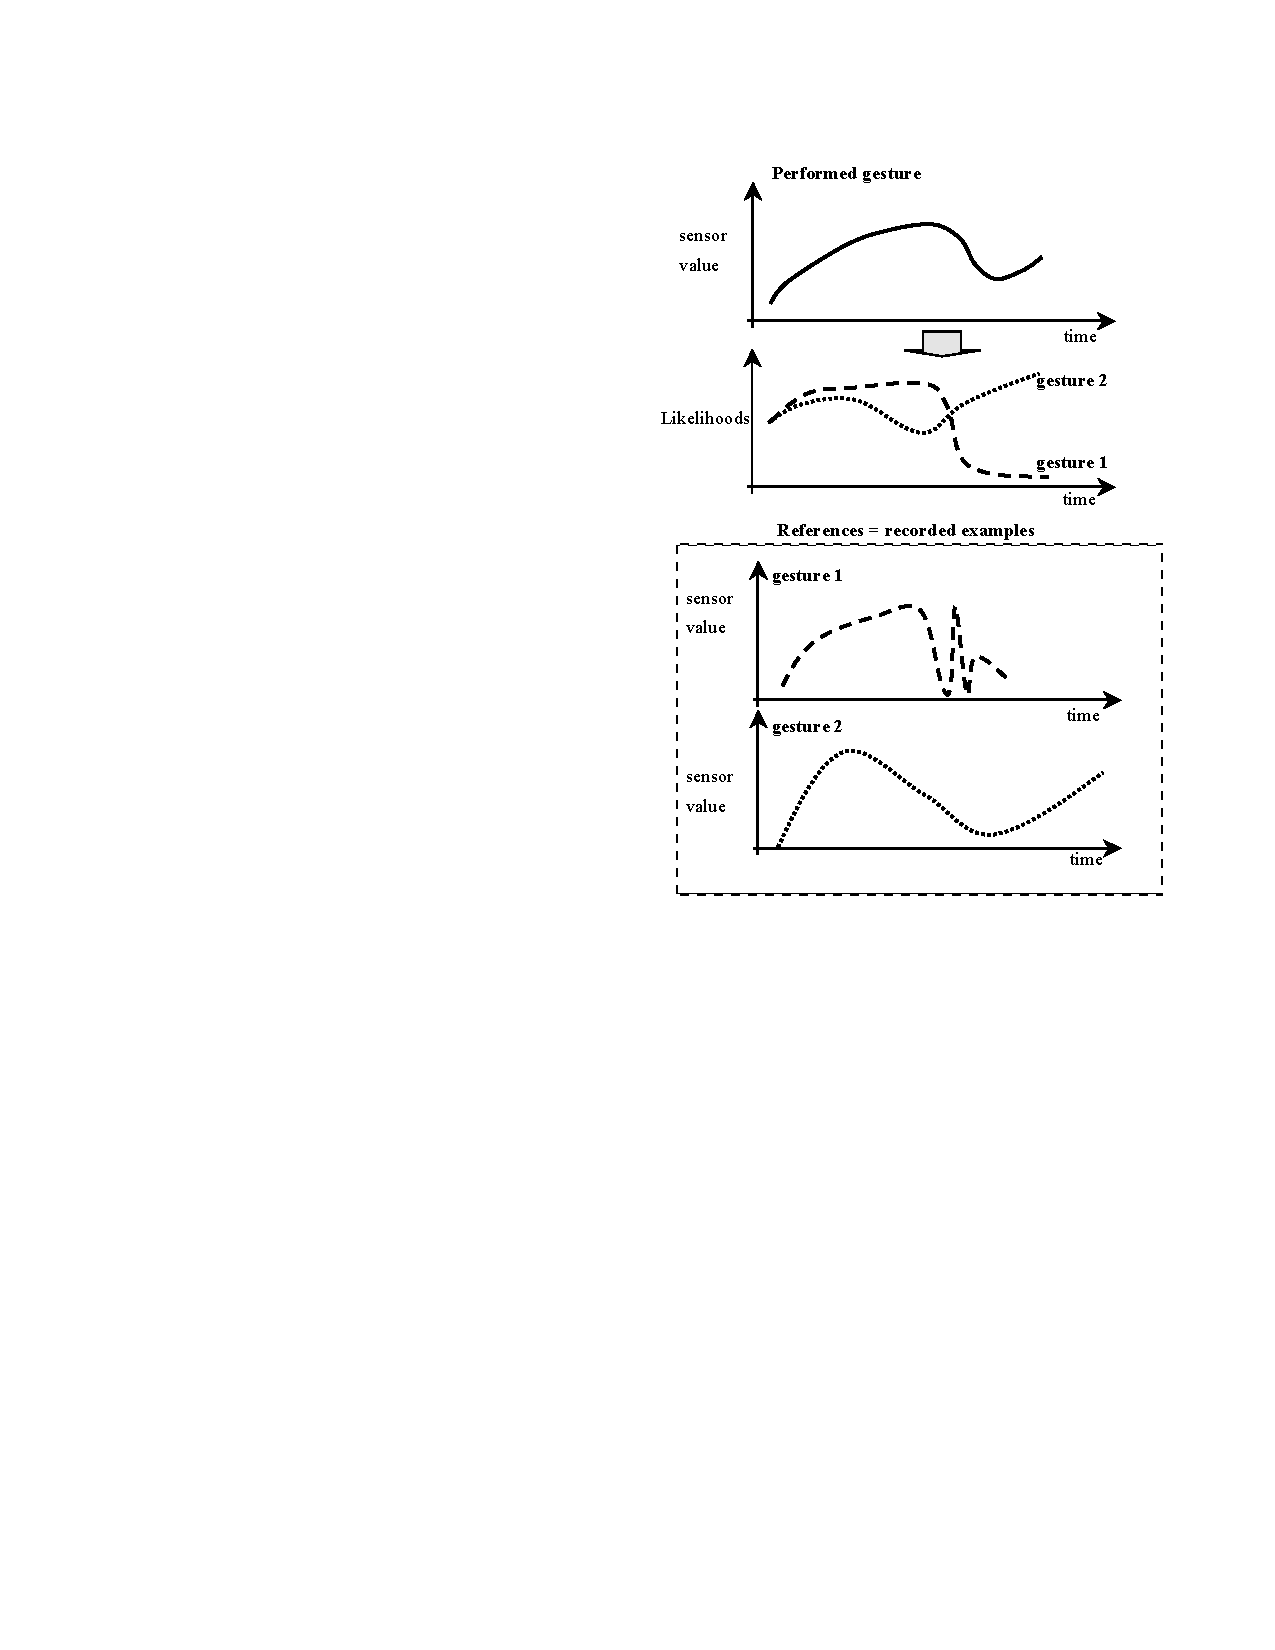
\includegraphics[scale=1.]{fig3.pdf}
%
% If no graphics program available, insert a blank space i.e. use
%\picplace{5cm}{2cm} % Give the correct figure height and width in cm
%
\caption{Comparison and recognition paradigm.}
\label{Bevilacqua:fig3}       % Give a unique label
\end{figure}

\subsection{Algorithm}
The two paradigms we described above, following and recognition can be directly implemented using Hidden Markov Models (HMM) \cite{Rabiner:1989}. Generally, the parameters of Markov models are estimated using the Baum-Welch algorithm using a large set of examples. In our case, we choose a simplified learning method enabling the use of a single example to determine the model parameter. To achieve this, assumptions are made on the expected variations within a class of gesture. This procedure can lead to a suboptimal determination of the Markov Model parameters. However, the possibility of using only a single example represents a significant advantage in term of usage. 

\subsubsection{Learning}
The learning process is illustrated in Figure~\ref{Bevilacqua:fig4} where the temporal curve is modeled as left-to-right Markov chain. The learning example is first downsampled, typically by a factor 2, and each sample value is associated to a state of the Markov chain. Assuming a constant sampling rate, the left-to-right transition probabilities are constant and directly related to the downsampling factor. For example, in the case of downsampling of factor n, the transition probabilities are equal to $1/n$, ensuring the Markov chain to model adequately the temporal behavior of the learning example. 

The observation probability function for each state is considered to be a multidimensional Gaussian model with a mean $\mu_i$ and a variance and $\sigma_i^2$, where $i$ is the state number. The mean $\mu_i$ is set to the value of the recorded gesture. The variance value is a factor adjusted by the user, which must match approximately expected variations between the performed and recorded gestures. In most of our experiments we found that the variance value is not critical since the recognition is based on a comparison process. 

\begin{figure}[t]
%\sidecaption
\centering
% Use the relevant command for your figure-insertion program
% to insert the figure file.
% For example, with the graphicx style use
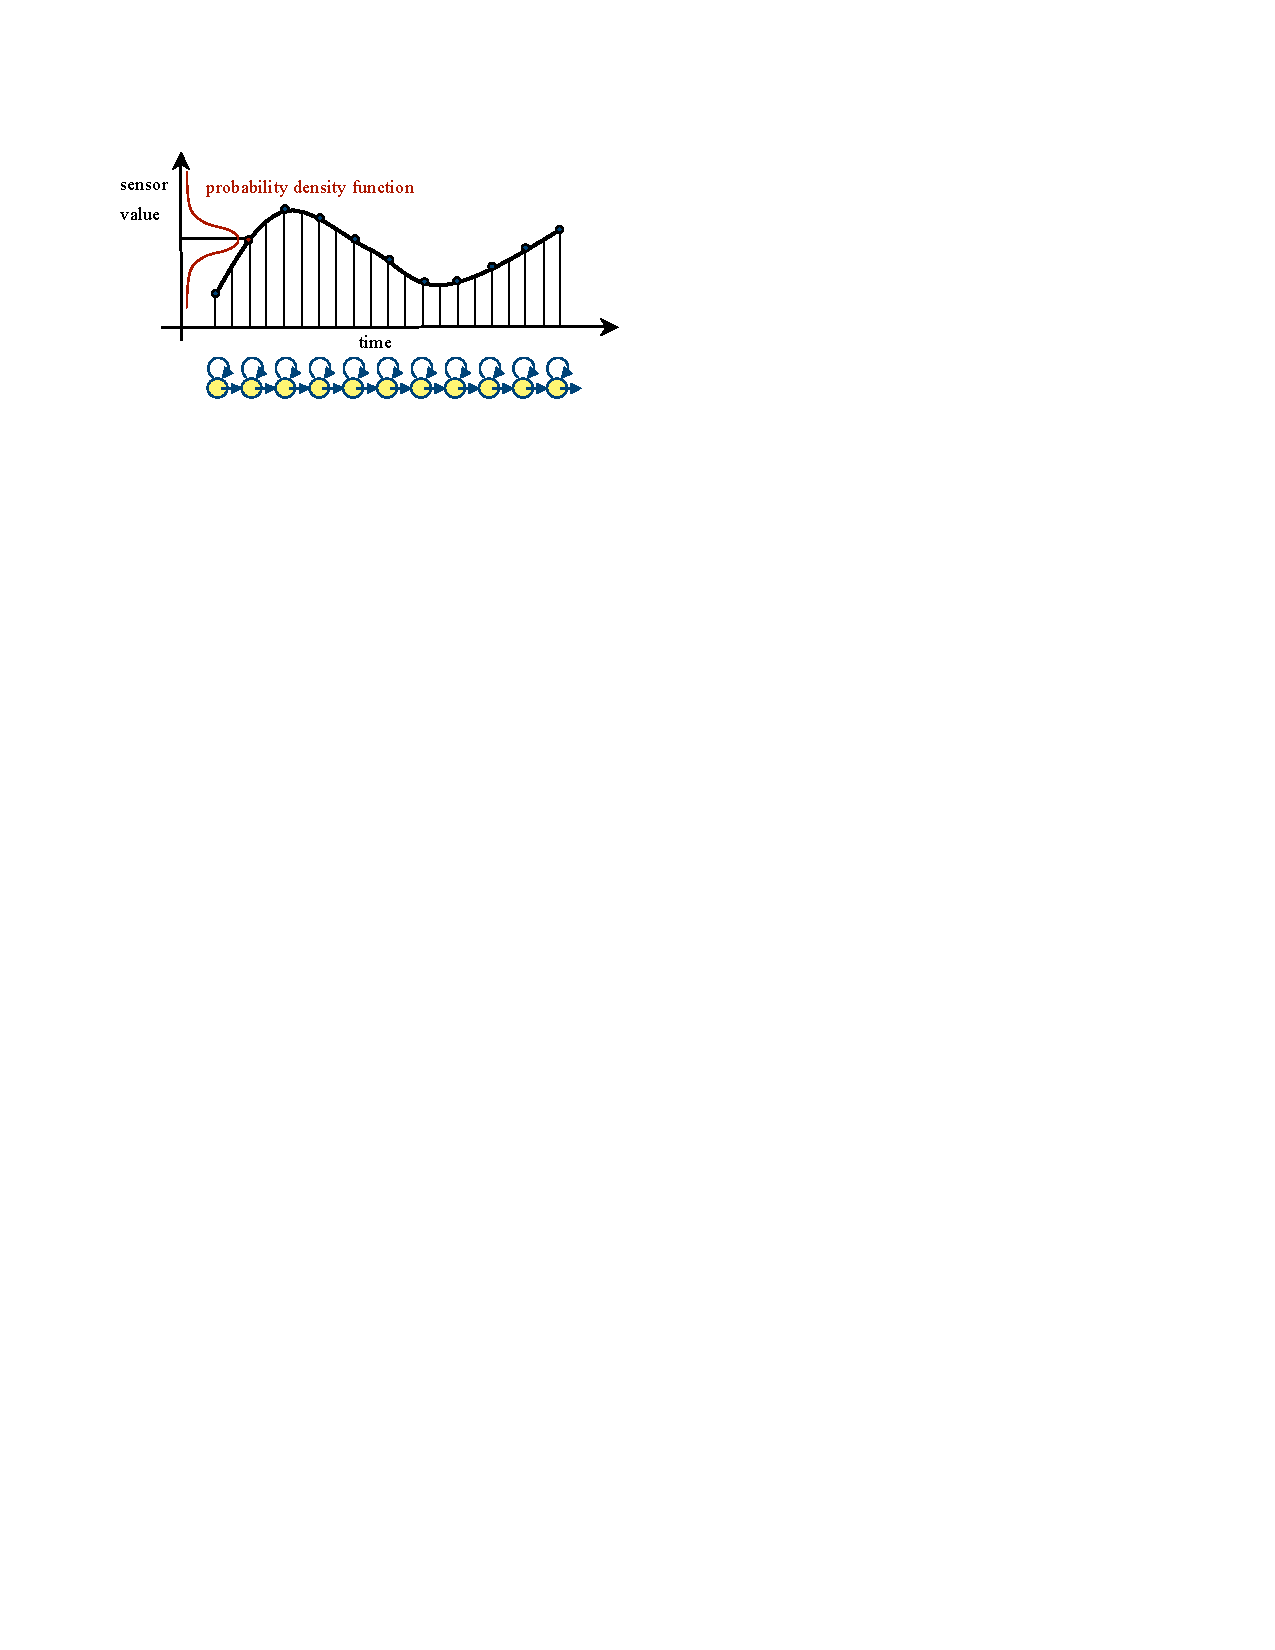
\includegraphics[scale=1.]{fig4.pdf}
%
% If no graphics program available, insert a blank space i.e. use
%\picplace{5cm}{2cm} % Give the correct figure height and width in cm
%
\caption{Learning procedure: a left-to-right HMM is used to model the example, down-sampled by a factor of 2.}
\label{Bevilacqua:fig4}       % Give a unique label
\end{figure}

\subsubsection{Decoding}
Consider the performed gesture as aN observation sequence $O_1..O_T$, corresponding to the performed gesture values from time $t = 1$ to $T $(sample index). The probability $\alpha_t(i)$ of  partial sequence (until time $t$) and state $i$ at time $t$ is computed from the standard forward procedure in HMM [19]. 
The following procedure corresponds to determine the most likely state $i$, denoted $m(t)$:%for all time $1...T$: 

 %
\begin{equation}
m(t)=\operatorname*{arg\,max}_i [\alpha_t(i)]\qquad 1 \leq t \leq T
\end{equation}
% 
Since the Markov chain has a simple left-to-right structure, the computed sequence of $m(t)$ reports time indexes of the time-warped sequence to the learned example (as shown in Figure~\ref{Bevilacqua:fig2}). 
The comparison and recognition procedure corresponds to compute the likelihood of the observation sequence for a given example (i.e. a given Markov model)

\begin{equation}
likelihood(i) = \sum_{i=1}^{N}\alpha_t(i)
\end{equation}
where $N$ is the number of states.

\subsubsection{Implementation}
The \emph{gesture-follower} is implemented as a set of Max/MSP modules integrated in the toolbox MnM \cite{Bevilacqua:2005} of the library FTM (LGPL licence) \cite{Schnell:2005a}. It takes advantages of the data structure of FTM for Max/MSP such as matrices and dictionaries. An example is freely available in the FTM package, under MnM/example.\footnote{This implementation is deprecated, please consider the freely available \emph{gf} external object in the MuBu package \url{http://forumnet.ircam.fr/fr/produit/mubu/}.}

\section{Pedagogical Experiments}
Conducting is an important part of musical education for all instrument players. It is an essential part of practice training, closely related to music theory. While teaching methods for small children or beginners are often based on playful approaches and exercises focusing on body movements (e.g. Dalcroze, Menuhin), music education at higher levels tends to underestimate these aspects. For some mid-level students, this may lead to a rigid posture and stiff gestures in their instrument practice. 

We performed two experiments with students during a regular music theory lesson (music school \emph{Atelier des Feuillantines} in Paris). Minimum perturbation was sought: the lesson was conducted by the usual teacher and following the usual lesson structure (Figure~\ref{Bevilacqua:fig5}). 

The pedagogical aim of the exercise was to experience and practice `smoothness' and `fluidity' of musical gestures. The prototype was used to continuously synchronise a chosen soundfile to a conducting gesture performed with the wireless module. The teacher starts the exercise by recording the reference gesture:  he conducts while listening to the soundfile. In a second phase, the students use the system to `conduct' the music, as further explained in the next section. 

\begin{figure}[t]
%\sidecaption
\center
% Use the relevant command for your figure-insertion program
% to insert the figure file.
% For example, with the graphicx style use
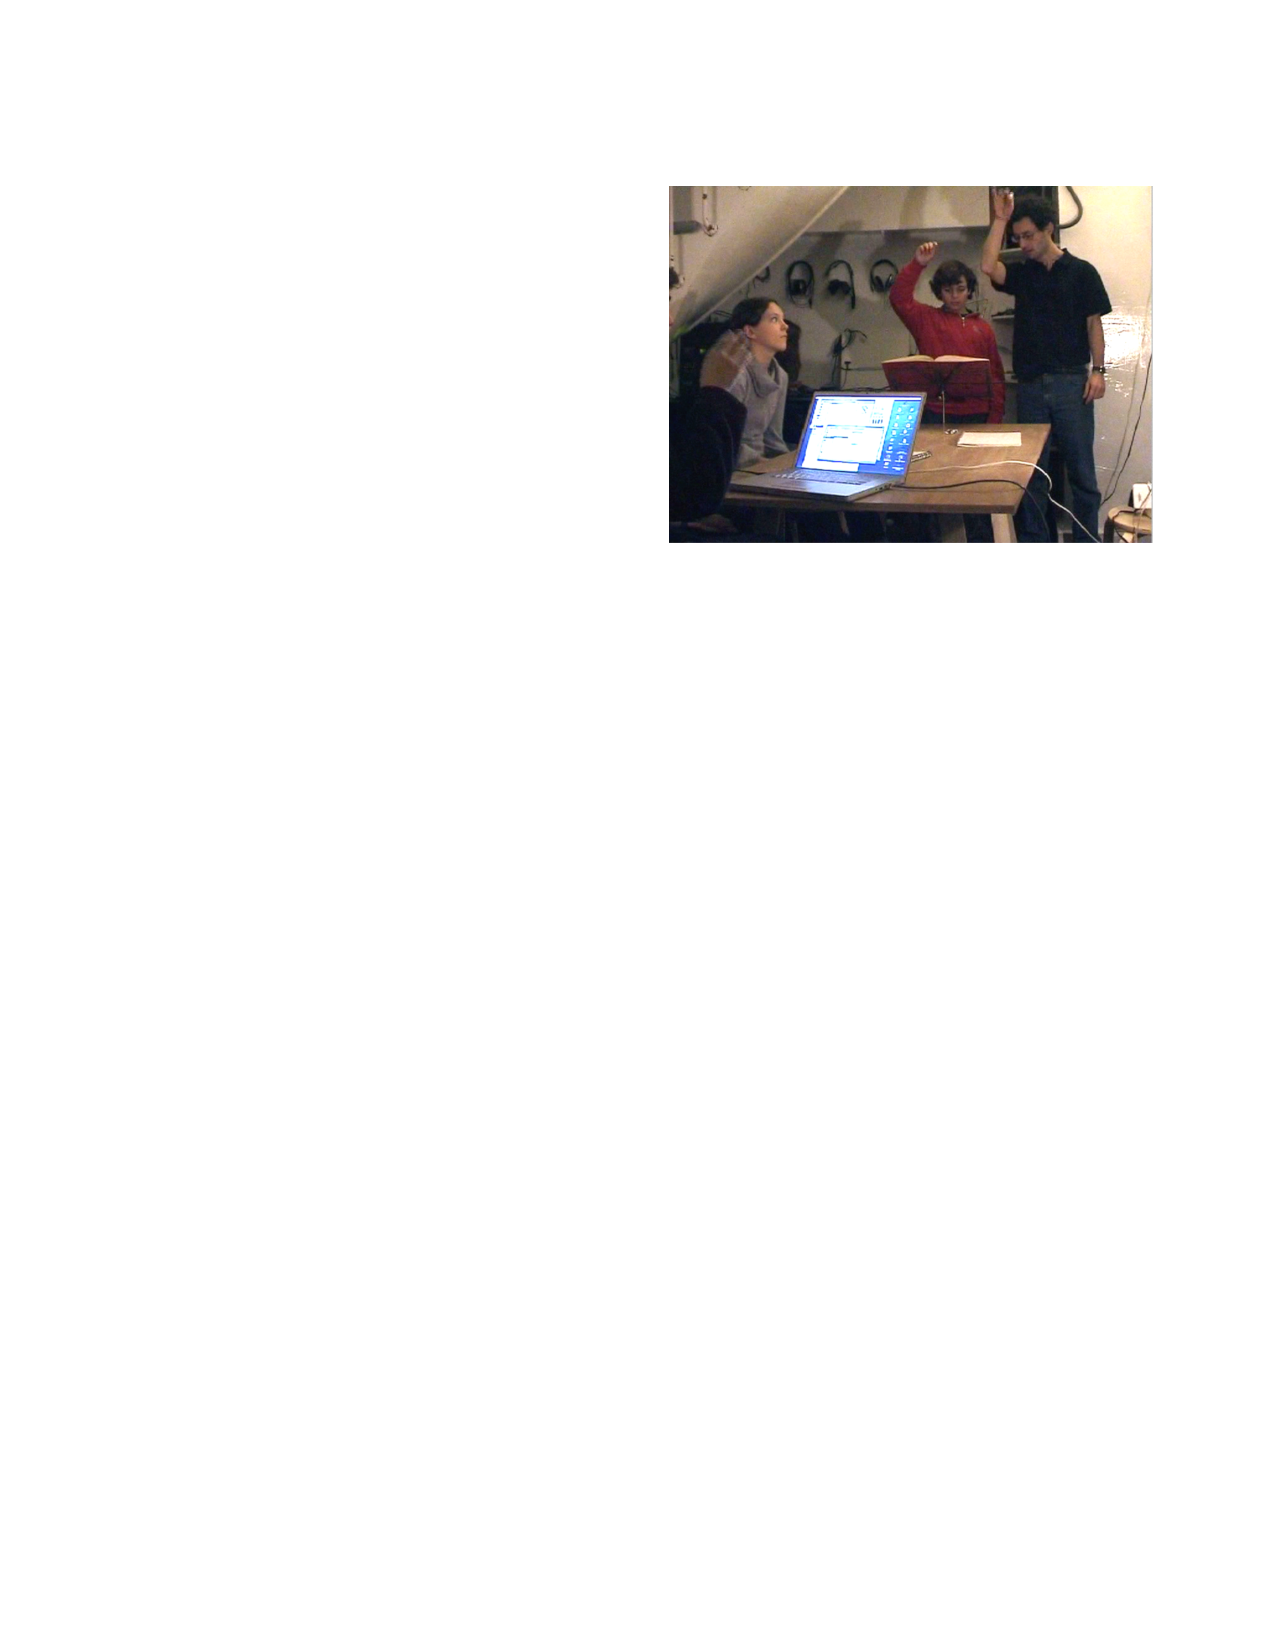
\includegraphics[scale=1.]{fig5.pdf}
%
% If no graphics program available, insert a blank space i.e. use
%\picplace{5cm}{2cm} % Give the correct figure height and width in cm
%
\caption{Teacher and student using the system during a music class. The teacher holds the wireless sensor module during the learning phase. }
\label{Bevilacqua:fig5}       % Give a unique label
\end{figure}

\subsection{Interaction paradigms}
The \emph{gesture-follower} was used to control the playback of soundfiles. The time index output by the \emph{gesture-follower} directly determines the position in the soundfile. Two types of time-stretching were used: granular synthesis or phase vocoder implemented with the Gabor library of FTM \cite{Schnell:2005,Schnell:2005a}.

On a practical level, the procedure is as follows:
\begin{enumerate}


\item Record mode: Record the gesture example while listening to the sound file. This step provides a gesture example that is synchronized with the soundfile. 
\item Play mode: The soundfile playback speed varies according to the \emph{gesture-follower} output, depending of the temporal variation in the gesture performance. 
\end{enumerate}

Separate soundfiles can be associated to different recorded examples. Different playback schemes are possible. First, the recognition feature can be used for the selection of the soundfile corresponding to the most likely gesture. Second, the different soundfiles can be played back simultaneously, and mixed according to the likelihood values.

This interaction paradigm can be used to simulate orchestral conducting. Similar applications have been proposed and implemented by several groups  \cite{Borchers:2006,Lee:2006,Lee:2006a}. However, our approach is distinct from those on various points. 

First, the gesture is considered here as a continuous process. In particular, no beat detection is used. This point has important consequences discussed in the next section. 

Second, the choice of the gesture is totally open and can be chosen with a very simple and effective procedure. As mentioned earlier, a single recording of the gesture is sufficient to operate the system. This flexibility allows us to elaborate pedagogical scenarios where the conducting pattern can be freely chosen and adjusted by the user. This point is further developed in section~\ref{Bevilacqua:sec:exp2}

\subsection{Experiment 1: Conducting}
After starting the software in \emph{record mode}, the teacher records a usual beat pattern gesture while listening to an excerpt of the soundfile. For example an excerpt of the Rite of Spring was chosen for its changes of metric.

The software is then switched in \emph{follow} mode and the students are asked to use the system to `conduct' the soundfile. An excerpt of a recorded beat pattern and the time-warped performed gesture is shown in Figure~\ref{Bevilacqua:fig6}. 

Since the system does track the entire gesture and not only the beats, the gesture between beats is important and affect directly the conducting procedure. Therefore, the audio playback speed depends directly on the overall movement quality. For example, if the student gesture does not match the smoothness and fluidity of the teacher gesture, a striking modification of the rhythmic pattern of the conducted sound appears (Figure~\ref{Bevilacqua:fig7}). This effect provides a direct sonic feedback to the students of its overall gesture quality, who can then progressively learn, `by ear,' how to perform a smooth and fluid gesture. 

\begin{figure}[t]
%\sidecaption
\center
% Use the relevant command for your figure-insertion program
% to insert the figure file.
% For example, with the graphicx style use
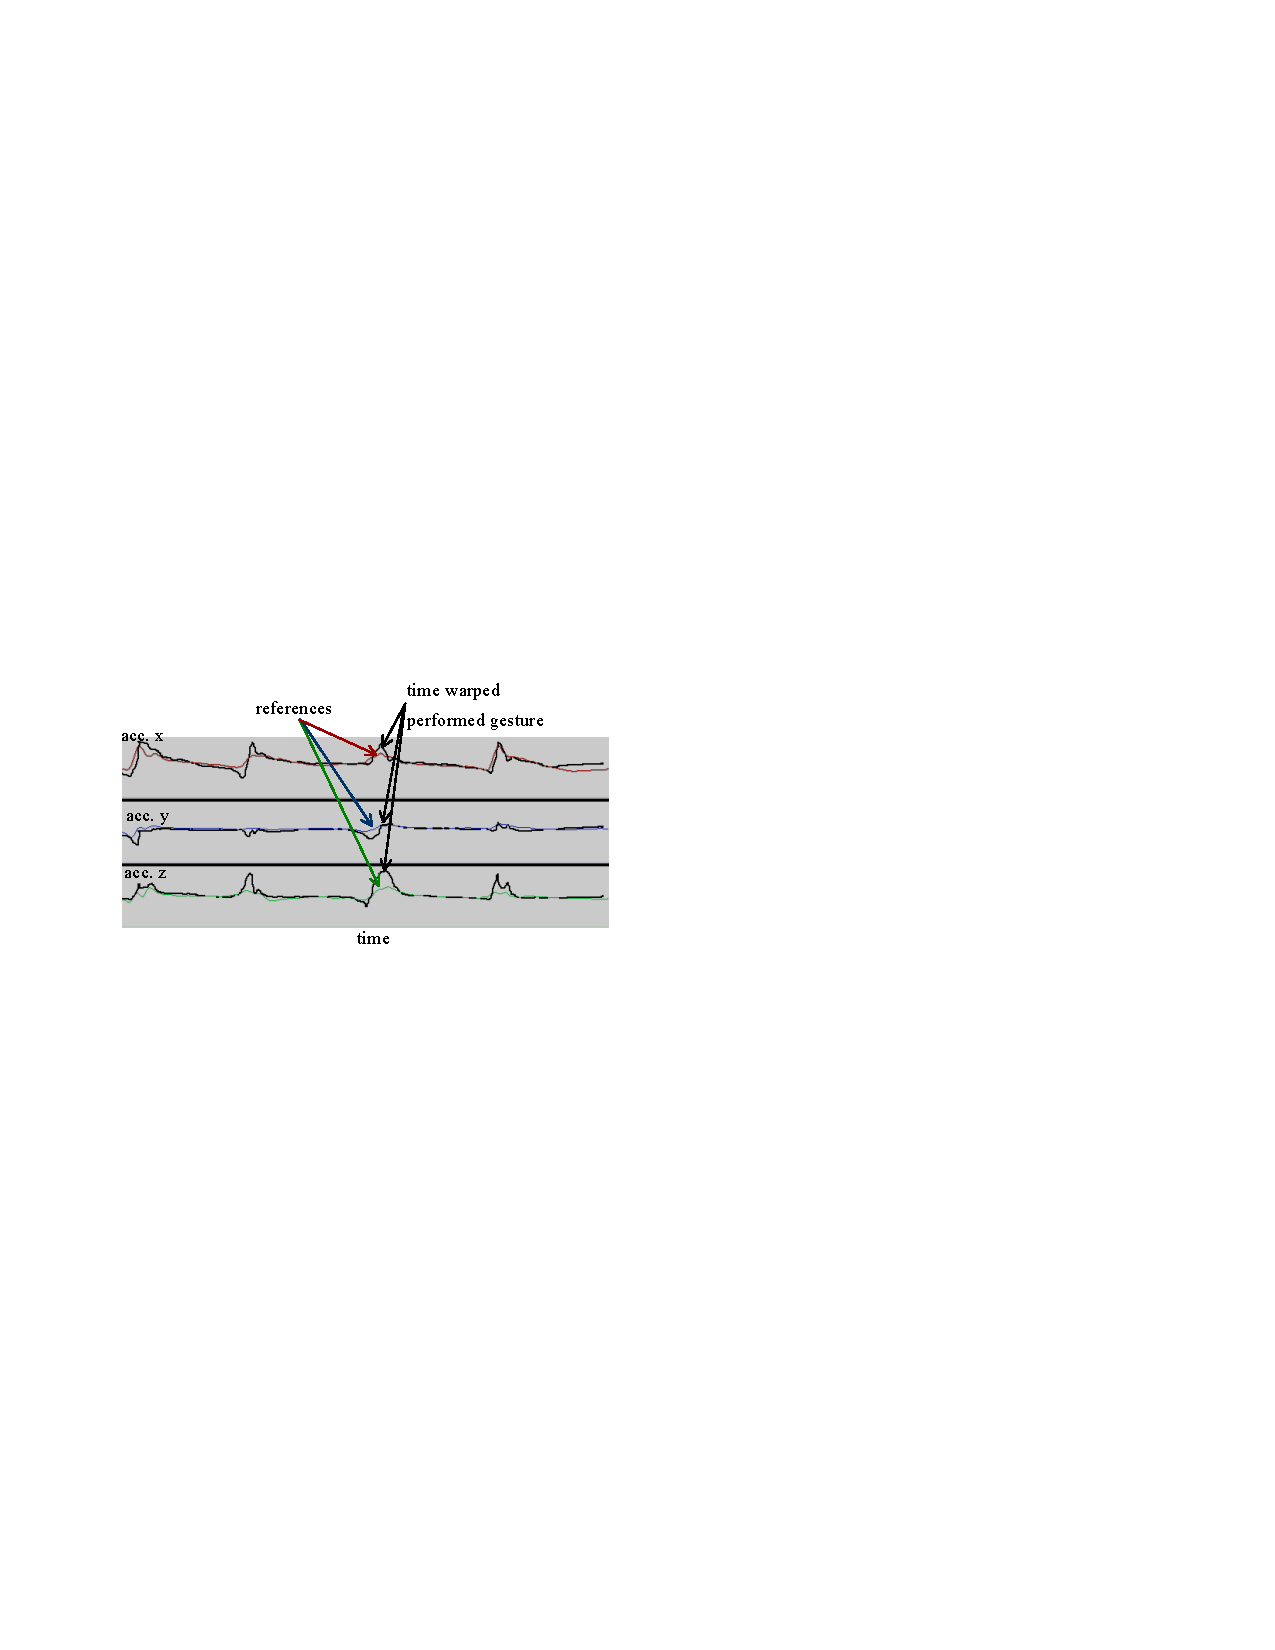
\includegraphics[scale=1.]{fig6.pdf}
%
% If no graphics program available, insert a blank space i.e. use
%\picplace{5cm}{2cm} % Give the correct figure height and width in cm
%
\caption{4-beat gesture as recorded by the 3D accelerometer. }
\label{Bevilacqua:fig6}       % Give a unique label
\end{figure}

\begin{figure}[t]
%\sidecaption
\center
% Use the relevant command for your figure-insertion program
% to insert the figure file.
% For example, with the graphicx style use
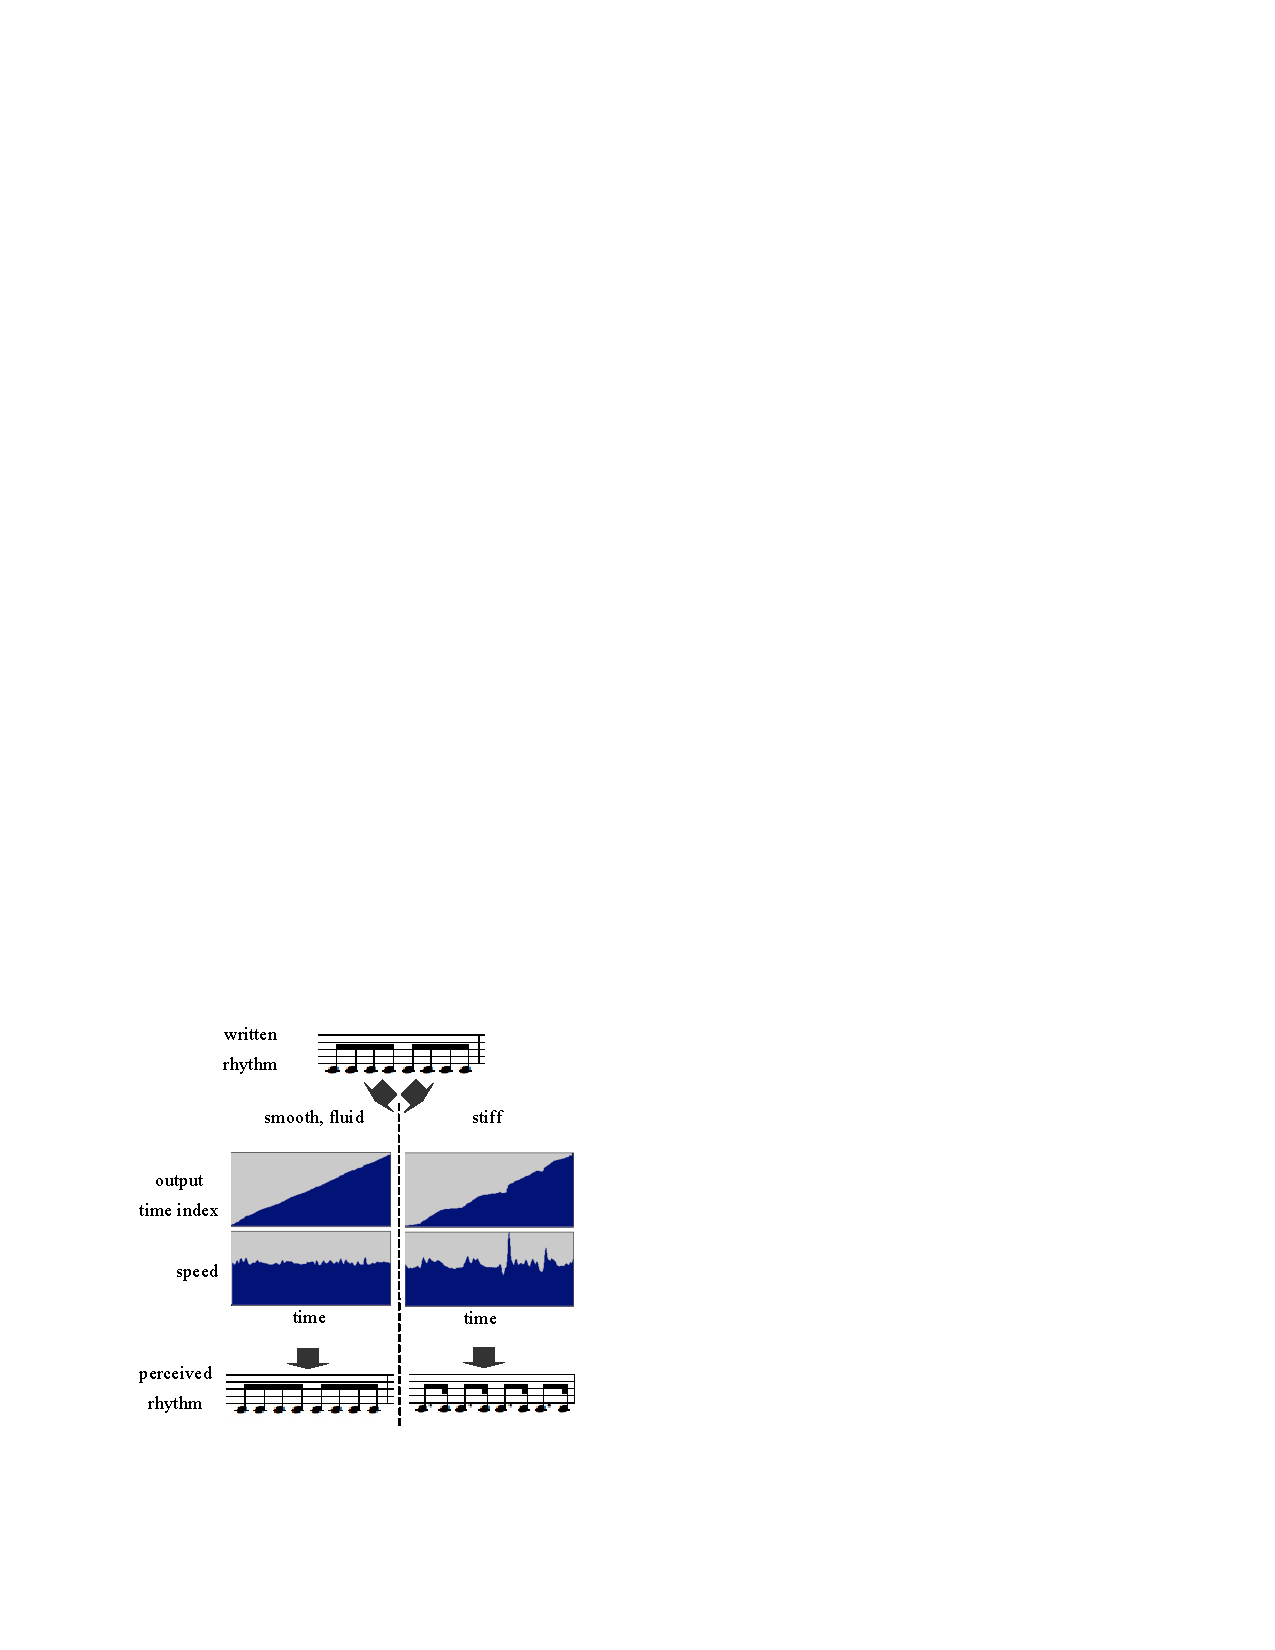
\includegraphics[scale=1.]{fig7.pdf}
%
% If no graphics program available, insert a blank space i.e. use
%\picplace{5cm}{2cm} % Give the correct figure height and width in cm
%
\caption{Effect of smoothness and fluidity in the performance of the 4-beat conducting pattern. }
\label{Bevilacqua:fig7}       % Give a unique label
\end{figure}


\subsection{Experiment 2: Free Gesture Exploration}
\label{Bevilacqua:sec:exp2}

In this experiment, the students were asked to find a free gesture they felt appropriate to various soundfiles. Various gestures were experimented by the students to control the temporal flow of music/sound. 

Different cases were tested, including the excerpts used for experiment 1. After experiencing traditional beating patterns, the students were able to try other types of gesture than usual conducting gestures. Voice recordings of the students were also used. The association of a free gesture to a voice recording allowed them for instance to alter the rhythm/prosody.

\subsection{Discussion and further work}
The experiments reported here must be understood as exploratory, and any definite conclusion should be avoided at this early stage. Importantly, the approach proposed here should be understood as complementary to traditional music teaching (rather than a replacement). The system was first tested during regular music theory lessons and the students were highly motivated by the experiments. Moreover, they immediately pointed out its creative potential. The teacher felt significant improvements of student awareness to key aspects of performance practice, for example musical phrasing. We summarise below important points that the experiments brought out, defining interesting paths for future work. 

\subsubsection{Smoothness and fluidity}
To experience smoothness and fluidity in a musical context was one of the goals of experiment 1. The control of these `gesture qualities' is crucial in music performance and interpretation, and represents generally a difficulty for young students. As a matter of fact, a usual problem among beginners (typically older than 10 years) resides in their overall body rigidity; they tend to move only the body parts touching the instrument. We found that our system was an interesting approach to stimulate adequate motion. Further experiments will concern attaching sensors to different body parts.

\subsubsection{Breathing}
Breathing is a well-known issue in music practice (directly linked to the point previously discussed). For example, students practicing `mechanically' in a stiff position tend to play often in apnoea, blocking their breathing.  These moments of apnea are evidence of insufficient connections between breathing and playing. The two experiments suggest that the system could be used to sonify particular gesture aspects directly linked to breathing and therefore helping the practice of musical phrasing/breathing.

\subsubsection{Link between intention and gesture}
The understanding of the musical structure and other compositional aspects of a musical piece (cadences for instance) usually help music interpretation and expression. Lack of theory understanding prevent students to elaborate consistent music interpretation. Our approach can potentially give opportunities to experience in an interactive way some aspects of music theory. 

\section{Conclusion}
We presented a set of hardware and software tools that were integrated in a fully functional prototype. On the technological side, the developments were found to be robust, and allowed for rapid prototyping of pedagogical experiments. A single person was able to install and operate the system seamlessly.

The first use of the system in a music class was encouraging and allowed us to confirm our approach. Larger scale experiments are currently planned with additional sound processing possibilities, including various sound synthesis modules. The same wireless sensor system and the \emph{gesture-follower} are currently adapted to the case of violin playing.


%
\begin{acknowledgement}
The I-MAESTRO project is partially supported by the European Community under the Information Society Technologies (IST) priority of the 6th Framework Programme for R\&D (IST-026883). Thanks to all I-MAESTRO project partners and participants, for their interests, contributions and collaborations.
We would like to thank Remy M\"uller, Alice Daquet, Nicolas Rasamimanana, Riccardo Borghesi, Diemo Schwarz and Donald Glowinski for contributions to this work and fruitful discussions.
\end{acknowledgement}
%

\section*{Author Commentary: Once Upon A NIME}

\paragraph{Frederic Bevilacqua and Norbert Schnell}

The initial aim of this article was to give an overview of research on music pedagogy with tangible interfaces that we were starting at that time in our team. The article contains three fairly independent contributions that alternatively could have been separated into three different articles:

\begin{itemize}
\item Wireless sensing hardware
\item Gesture analysis and interactive machine learning software
\item Applications and use cases in music pedagogy
\end{itemize}

However, the idea was to describe how different streams of NIME research converged in specific use cases that had been actually implemented. Revisiting the three themes almost 10 years later gives the opportunity to contextualize this work in the flow of still ongoing research and development.

Firstly, the possibility to create a small size wireless sensor interface using off-the-shelf wireless transmission modules marked a considerable breakthrough compared to other systems we reported earlier in the NIME community (see \cite{Flety:2011} and references herein). The advantage of these modules resided in the favorable compromise between a small size, low power consumption and relatively high bandwidth. Moreover, it was possible to use several wireless interfaces in parallel. This matched well with our applications that included music and dance performance as well as experimental music pedagogy. This hardware development, among others at the time, was representative of the increased use of wireless technology at NIME. For our research group, this development allowed us to boost the use of miniature wireless interfaces using inertial measurement units, such as accelerometers and gyroscopes. Since then, we have employed different generations of such IMU-based wireless interface in many applications that more recently also include mobile and web platforms. In fact, the development described in the article coincides with that of the first generation of smartphones as well as the first generation of game controllers that include wireless motion sensing such as the Wiimote (with a much bigger form factor and still lacking precision and reliability).

Secondly, this article featured the first complete description of the ``gesture follower,'' which represents an important line of research in our team until now. The gesture follower has been used since this reports in a large number of artistic performances and installations, in music and dance \cite{Bevilacqua:2011}. More complete descriptions followed in subsequent articles and this research influenced similar methods such as ``Mapping by Listening'' and tools such as GVF \cite{Caramiaux:2014} or even more recently XMM \cite{Francoise:2014}. The gesture follower can be considered as our first development in what we call now more generally ``interactive machine learning'' (but the name was not as common in NIME at that time). In particular, it allowed users to record, as many time they wanted, their gestures to build movement-sound interactions based on rather few examples. We found this flexibility a key element for the music pedagogy use cases we reported on as well as for many other use cases we developed over the past years.
Finally, the applications in music education described in the article occupied us for several years of continued research. These ``real-world'' applications certainly contributed to foster several concepts we're pursuing, such as the use of ``metaphors'' and ``playing techniques.''

Globally, this proceeding can be seen as the start of a line of research that produced our interface MO---Modular Musical Objects, that were also reported in the NIME community \cite{Schnell:2011} and that also won the Margaret Guthman Musical Instrument Competition.\footnote{\url{http://guthman.gatech.edu/}} Many of the ideas and techniques that were presented in this article are still actively pursued, in particular with mobile and web technologies.


\section*{Expert Commentary: Gesture Following Made Accessible}

\paragraph{Kristian Nymoen}

One of the beauties of the NIME conference is the encouragement of publications that focus on novel systems for musical expression. As a result, many NIME publications are often broad in scope, presenting an entire system, including the hardware, software, modes of interaction, musical output, and more. Sometimes the presented system as a whole persists as a symbolic interface for musical expression for many years to come. In other cases a particular sub-unit of the system, such as a piece of hardware or a specific mode of interaction, is the contribution that makes the publication leave its mark within and beyond the community. 

The paper by Bevilacqua et al. demonstrates brilliantly how NIME developments may provide important outcomes. The paper is ``disguised'' as a well-written, yet quite ordinary, NIME paper on a prototype of a complete system for music pedagogy. The custom-made hardware was thoroughly documented and a cutting edge solution for portable sensing and wireless communication. The proposed problem of using technology for studying and teaching fluidity in conducting is still relevant, and the authors showed the applicability of the system for this task through testing and evaluating in a real pedagogical context with students and their teacher. Still, it is the software part of the system that really stands out as one of the important NIME contributions of the decade: the ``Gesture Follower.''

The Gesture Follower was implemented in IRCAM's FTM framework for Max. The FTM framework extends Max with various types of data structures and operators, and facilitates many types of data processing in Max, for instance of motion data. The implementation in Max is one of the main reasons why the Gesture Follower became such an important piece of software. Gesture recognition in music had already been explored for several years at the time of this paper's publication. However, its application required knowledge of the machine learning algorithms involved and in most cases also proficiency in some text-based programming environment. The out-of-the-box examples and tutorials for the Gesture Follower made gesture recognition accessible to a larger user-group, including musicians and artists who preferred the graphical interface of Max to text-based languages. 

Not only was the Gesture Follower more accessible due to its Max implementation, it provided a combination of highly useful features for use in musical interaction. Classification happens in real time, continuously updating the classification score against each of the pre-trained examples while the user is moving. As such, the system can easily be used in mapping between motion data and synthesizer parameters. To allow for different durations between training examples and the input gestures, an elegant time-warping solution has been implemented. For each of the pre-trained examples, the Gesture Follower provides an estimation of the time index within the gesture. In other words, the system does not only recognize the gesture, it \emph{follows} the gesture. With such a time warping function in place, it is possible match the playback duration to the duration of the input gesture.

Since this first publication on the Gesture Follower, the IRCAM team has presented a number of follow-up articles with various improvements and testing of the system in different contexts \cite{Bevilacqua:2010,Bevilacqua:2012}. One of the developments is the implementation of the Gesture Follower in IRCAM's multi-buffer solution for audio and motion capture data in Max, Mubu, with improvements in both functionality and user interface. 

The paper of Bevilacqua et al. shows that developing new interfaces for musical expression is more than just developing a system in itself. NIME technologies are often highly generic, and may have much broader application areas than the system that is presented in the NIME publication. In this specific case, the Gesture Follower was presented as one part of a system for music pedagogy, but has proven just as useful in music performance \cite{Van-Nort:2013}, specialized systems for multimodal score-following \cite{Ritter:2013}, or even tasks unrelated to music, such as recognition of wheel-throwing pottery gestures \cite{Manitsaris:2014}.

